

% All information flows point from sender to receiver; see notation key.
\begingroup
\definecolor{archline}{HTML}{2F425A}
\definecolor{archtext}{HTML}{1E293B}
\definecolor{aiborder}{HTML}{1261A8}
\definecolor{aifill}{HTML}{DCEBFE}
\definecolor{knowborder}{HTML}{26864A}
\definecolor{knowfill}{HTML}{E1F4E5}
\definecolor{verborder}{HTML}{3F2C8C}
\definecolor{verfill}{HTML}{EAE6FA}
\definecolor{execborder}{HTML}{B86F00}
\definecolor{execfill}{HTML}{FEEDCD}
\definecolor{extborder}{HTML}{44556B}
\definecolor{extfill}{HTML}{DCDDE2}

\usetikzlibrary{arrows}
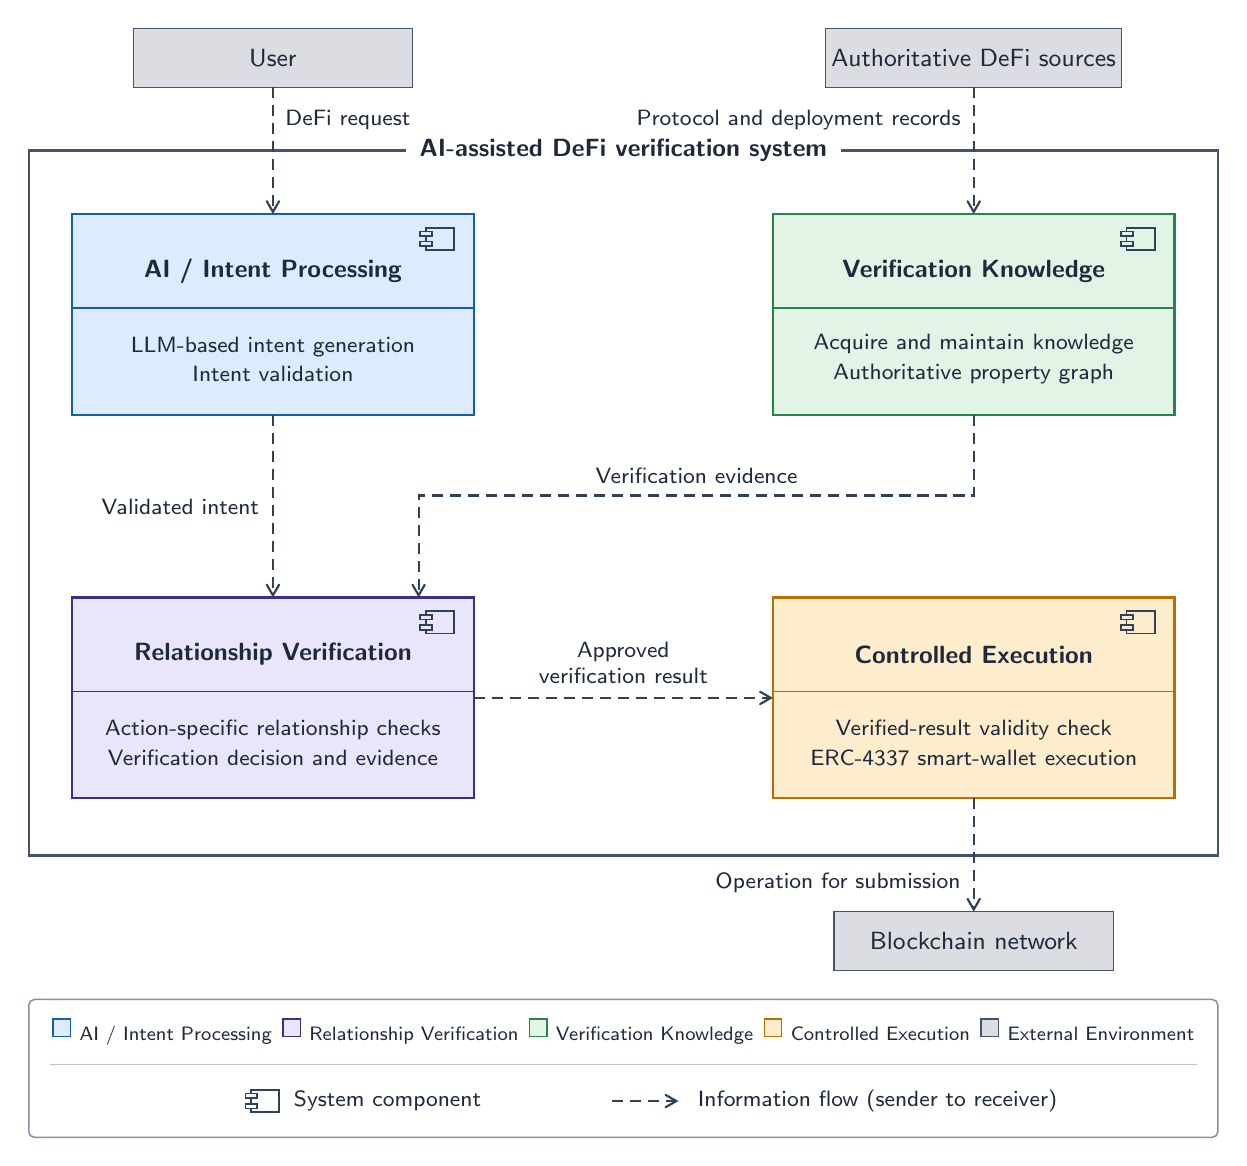
\begin{tikzpicture}[x=1cm,y=1cm,
 every node/.style={text=archtext,font=\sffamily\small,align=center},
 infoflow/.style={->,>=angle 60,draw=archline,dash pattern=on 4pt off 2.5pt,line width=.78pt},
 assoc/.style={draw=archline,line width=.78pt},
 labeltext/.style={font=\sffamily\footnotesize,inner sep=2pt},
 ext/.style={draw=extborder,fill=extfill,minimum width=3.55cm,
   minimum height=.75cm,inner sep=2pt,outer sep=0pt}]
% UML component glyph: a classifier rectangle with two protruding tabs.
\def\ArchGlyph#1#2#3{%
  \begin{scope}[shift={(#1,#2)},draw=archline,line width=.6pt]
    \draw[fill=#3] (-.18,-.14) rectangle (.18,.14);
    \draw[fill=#3] (-.25,.035) rectangle (-.10,.095);
    \draw[fill=#3] (-.25,-.095) rectangle (-.10,-.035);
  \end{scope}}
% The four equal component symbols have a header and a responsibility list.
% Parameters: name, x, y, outline, fill, title, responsibilities.
\def\ArchComponent#1#2#3#4#5#6#7{%
  \node[rectangle,draw=#4,fill=#5,line width=.85pt,
     minimum width=5.10cm,minimum height=2.55cm,inner sep=0pt,
     outer sep=0pt] (#1) at (#2,#3) {};
  \begin{scope}[shift={(#1.center)}]
    \ArchGlyph{2.12}{.96}{#5}
    \node[font=\sffamily\bfseries\small,inner sep=0pt] at (0,.55) {#6};
    \draw[draw=#4,line width=.55pt] (-2.55,.08) -- (2.55,.08);
    \node[inner sep=0pt,font=\sffamily\fontsize{8.1}{10.8}\selectfont] at (0,-.57) {#7};
  \end{scope}}
\draw[draw=extborder,line width=.85pt] (0,1.7) rectangle (15.1,10.65);
\node[anchor=center,fill=white,inner xsep=5pt,font=\sffamily\bfseries\small]
 at (7.55,10.65) {AI-assisted DeFi verification system};

\ArchComponent{ai}{3.1}{8.57}{aiborder}{aifill}{AI / Intent Processing}
  {LLM-based intent generation\\Intent validation}
\ArchComponent{knowledge}{12.0}{8.57}{knowborder}{knowfill}{Verification Knowledge}
  {Acquire and maintain knowledge\\Authoritative property graph}
\ArchComponent{verifier}{3.1}{3.70}{verborder}{verfill}{Relationship Verification}
  {Action-specific relationship checks\\Verification decision and evidence}
\ArchComponent{exec}{12.0}{3.70}{execborder}{execfill}{Controlled Execution}
  {Verified-result validity check\\ERC-4337 smart-wallet execution}

% External entities.
\node[ext] (user) at (3.1,11.83) {User};
\node[ext] (sources) at (12,11.83) {Authoritative DeFi sources};
\node[ext] (chain) at (12,.61) {Blockchain network};

% Labels identify the information conveyed, rather than the calling component.
\draw[infoflow] (user.south) -- (ai.north);
\node[labeltext,anchor=west] at (3.18,11.04) {DeFi request};
\draw[infoflow] (sources.south) -- (knowledge.north);
\node[labeltext,anchor=east] at (11.91,11.04) {Protocol and deployment records};

% The verifier has two independent inputs, with distinct arrow endpoints.
\draw[infoflow] (ai.south) -- (verifier.north);
\node[labeltext,anchor=east] at (3.00,6.13) {Validated intent};
\draw[infoflow] (knowledge.south) -- (12.0,6.27) -- (4.95,6.27)
  -- (4.95,4.975);
\node[labeltext,anchor=south] at (8.48,6.34) {Verification evidence};
\draw[infoflow] (verifier.east) -- (exec.west);
\node[labeltext,anchor=south] at (7.55,3.80) {Approved\\verification result};
\draw[infoflow] (exec.south) -- (chain.north);
\node[labeltext,anchor=east] at (11.91,1.35) {Operation for submission};

% One-row colour legend, with a separate notation key underneath.
\draw[draw=extborder!65,rounded corners=2pt,line width=.55pt]
  (0,-1.88) rectangle (15.10,-.13);
\def\ArchSwatch#1#2{%
  \tikz[baseline=-.48ex]{\draw[draw=#1,fill=#2,line width=.55pt]
       (0,0) rectangle (.22,.22);}\hspace{3pt}}
\node[inner sep=0pt,font=\sffamily\fontsize{7.4}{9.2}\selectfont]
 at (7.55,-.54) {\makebox[14.50cm][s]{%
  \ArchSwatch{aiborder}{aifill}AI / Intent Processing\hfill
  \ArchSwatch{verborder}{verfill}Relationship Verification\hfill
  \ArchSwatch{knowborder}{knowfill}Verification Knowledge\hfill
  \ArchSwatch{execborder}{execfill}Controlled Execution\hfill
  \ArchSwatch{extborder}{extfill}External Environment}};
\draw[draw=extborder!35,line width=.4pt] (.27,-.96) -- (14.83,-.96);
\ArchGlyph{3.0}{-1.42}{white}
\node[labeltext,anchor=west] at (3.29,-1.42) {System component};
\draw[infoflow] (7.41,-1.42) -- (8.25,-1.42);
\node[labeltext,anchor=west] at (8.42,-1.42)
  {Information flow (sender to receiver)};
\end{tikzpicture}
\endgroup